\documentclass{standalone}
\usepackage{tikz}
\usetikzlibrary{decorations.pathmorphing}
\definecolor{la_white}{RGB}{233,235,223} %#E9EBDF
\definecolor{la_dark}{RGB}{59,54,81}     %#3B3651
\definecolor{la_gray}{RGB}{96,112,139}   %#60708B
\definecolor{la_tan}{RGB}{152,159,122}   %#989F7A

\begin{document}
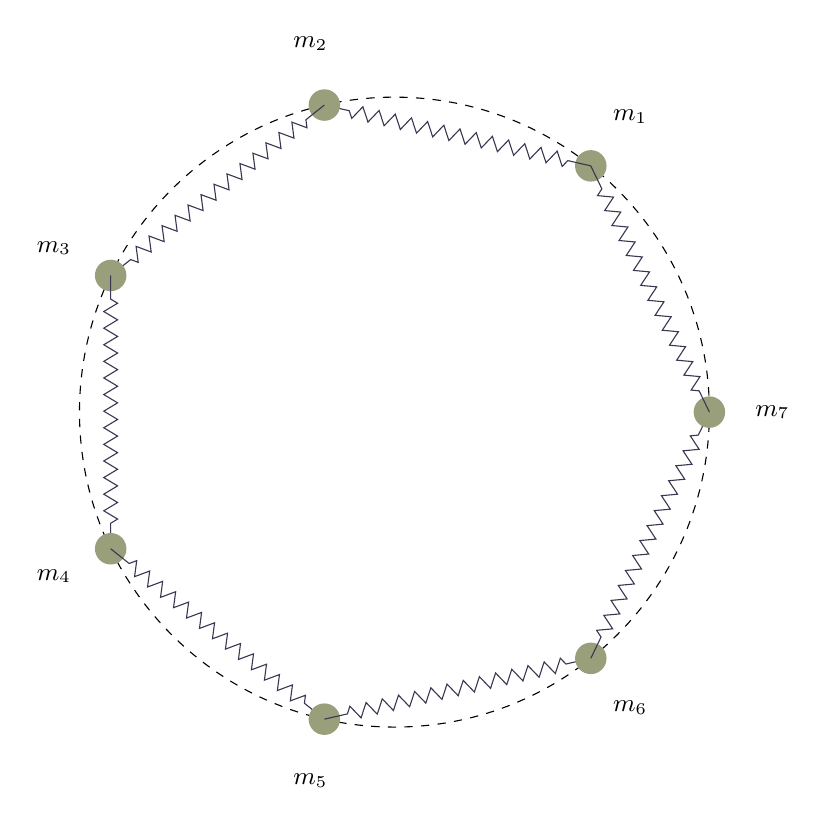
\begin{tikzpicture}[scale=2]
    % Define spring style
    \tikzset{spring/.style={decorate,decoration={zigzag,pre length=0.3cm,post length=0.3cm,segment length=6}}}

    \draw[dashed] (0,0) circle (2cm); % Draw the circle

    \pgfmathsetmacro{\angle}{360/7}   % Calculate angle between masses


    \foreach \i in {1,...,7}    % Draw masses and springs
    {
        % Calculate position
        \pgfmathsetmacro{\x}{2*cos(\i*\angle)}
        \pgfmathsetmacro{\y}{2*sin(\i*\angle)}
        
        % Draw mass
        \fill[color=la_tan] (\x,\y) circle (0.1cm);
        \node[font=\small] at ({\x*1.2},{\y*1.2}) {$m_{\i}$};
        
        % Draw spring to next mass
        \pgfmathsetmacro{\nextx}{2*cos((\i+1)*\angle)}
        \pgfmathsetmacro{\nexty}{2*sin((\i+1)*\angle)}
        \draw[spring,color=la_dark] (\x,\y) -- (\nextx,\nexty);
    }
\end{tikzpicture}
\end{document}
